
Oppgavetekst
Now set up a test of the conditioning of the GPS problem. Define satellite positions $(A_i,B_i,C_i)$ from spherical coordinates $(\rho,\phi i,\theta i)$ as

\begin{align}
	A_i &= \rho \cos{\phi i} \cos{\theta i} \nonumber \\
	B_i &= \rho \cos{\phi i} \sin{\theta i} \nonumber \\
	C_i &= \rho \sin{\theta i} \nonumber \\
\end{align}

where $\rho = 26570$ km is fixed, while $0 \leq \phi_i \leq \frac{\pi}{2}$ and $0 \leq \theta_i \leq 2 \pi$ for $i=1,...,4$ are chosen arbitrarily. The $\phi$ coordinate is restricted so that the four satellites are in the upper hemisphere. Set $x = 0$, $y = 0$, $z = 6370$, $d = 0.0001$, and calculate the corresponding satellite ranges $R_i = \sqrt{A_i^2 + B_i^2 + (C_i − 6370)^2}$ and travel times $t_i = d + R_i /c$.

We will define an error magnification factor specially tailored to the situation. The atomic clocks aboard the satellites are correct up to about 10 nanoseconds, or $10^{−8}$ second. Therefore, it is important to study the effect of changes in the transmission time of this magnitude. Let the backward, or input error be the input change in meters. At the speed of light, $t_i = 10^{−8}$ second corresponds to $10^{−8}c \approx 3$ meters. Let the forward, or output error be the change in position $||(\Delta x,\Delta y,\Delta z)||_\infty$, caused by such a change in $t_i$, also in meters. Then we can define the dimensionless 

\begin{align}
    \text{error magnification factor} = \frac{||(\Delta x,\Delta y,\Delta z)||_\infty}{c||(\Delta t_1,...,\Delta t_m)||_\infty} \nonumber
\end{align}

and the condition number of the problem to be the maximum error magnification factor for all small $\Delta t_i$ (say, $10^{−8}$ or less).

Change each $t_i$ defined in the foregoing by $t_i = +10^{-8}$or $−10^{−8}$, not all the same. Denote the new solution of the equations (4.37) by $(\bar{x},\bar{y},\bar{z},\bar{d})$, and compute the difference in position $||(\Delta x,\Delta y,\Delta z)||_\infty$ and the error magnification factor. Try different variations of the $\Delta t_i$'s. What is the maximum position error found, in meters? Estimate the condition number of the problem, on the basis of the error magnification factors you have computed. 

\textbf{Løsning}

\begin{lstlisting}[caption={task4.m},label=lst:task4.m]
function [conditionNumber, worst_max_pos_error] = task4()
	%definerer konstanter gitt i oppgaven, og lager tilfeldige punkter 
	%phi ogtheta
	rho = 26570;
	c = 299792.458;
	phi = [0.3, 1.2, pi/8, pi/6];
	theta = [1.2,2,3,4.5];

	%Lager vektorer A, B og C, og fyller inn verdiene gitt i oppgaven
	A = ones(1,4); 
	B = ones(1,4); 
	C = ones(1,4);

	for i=1:4
	    A(i) = rho * cos(phi(i)) * cos(theta(i));
	    B(i) = rho * cos(phi(i)) * sin(theta(i));
	    C(i) = rho * sin(phi(i));
	end

	%Lager en R- og t-vektor som definert i teksten
	R = sqrt((A.^2)+(B.^2)+((C-6370).^2));
	t = 0.0001 + (R/c);

	%Lager en riktig løsning, løst ved koden i task2general. 
	[x,y,z,d]= task2general(A,B,C,t); 
	riktig = [x y z d];

	%Definerer en matrise som inneholder alle mulige kombinasjoner av + og -
	%feil. 
	factor = [[-1,-1,-1,1];[-1,-1,1,1];[-1,1,1,1];[-1,1,-1,1];[-1,1,1,-1];[-1,-1,1,-1];[-1,1,-1,-1];[1,1,1,-1];[1,1,-1,-1];[1,-1,-1,-1];[1,-1,1,-1];[1,-1,-1,1];[1,1,-1,1];[1,-1,1,1]];


	max_pos_error = zeros(1,14);
	emf = zeros(1,14);

	%regner ut nye tider basert på faktorene, og løser problemet igjen med
	%task2general. Finner deretter ut den maksimale posisjonsfeilen, samt 
	%EMF for hver utregning.
	for i = 1:length(factor)
	    dt1(1) = t(1) + 1e-8*factor(i,1);
	    dt1(2) = t(2) + 1e-8*factor(i,2);
	    dt1(3) = t(3) + 1e-8*factor(i,3);
	    dt1(4) = t(4) + 1e-8*factor(i,4); 
	    [x2,y2,z2,d2]=task2general(A,B,C,dt1);
	    feil = [x2 y2 z2 d2];
	    max_pos_error(i) = max(abs(riktig-feil));
	    emf(i) = max_pos_error(i)/(c*max(abs(dt1-t)));
	end


	full(max_pos_error)
	full(emf)

	%Finner den største posisjonsfeilen og kondisjonstallet.
	worst_max_pos_error = max(full(max_pos_error));
	conditionNumber = max(emf);

end
\end{lstlisting}

\begin{lstlisting}[caption={task2general.m}]
function [x,y,z,d] = task2general(A, B, C, t)
	A1=A(1); 
	A2=A(2); 
	A3=A(3); 
	A4=A(4); 
	t1=t(1); 

	B1=B(1); 
	B2=B(2); 
	B3=B(3); 
	B4=B(4); 
	t2=t(2); 

	C1=C(1); 
	C2=C(2); 
	C3=C(3); 
	C4=C(4); 
	t3=t(3); 
	t4=t(4);
	%Lyshastigheten c

	c = 299792.458;

	% Definerer Ux, Uy og Uz som regnet ut i teorien 
	Ux = -2 *[A1 - A2; A1 - A3; A1 - A4];
	Uy = -2 *[B1 - B2; B1 - B3; B1 - B4];
	Uz = -2 *[C1 - C2; C1 - C3; C1 - C4];
	Ud = 2 *(c^2)*[t1 - t2; t1 - t3; t1 - t4];
	W = [A1^2 - A2^2 + B1^2 - B2^2 + C1^2 - C2^2 - (c^2)*(t1^2) + (c^2)*(t2^2); 
	     A1^2 - A3^2 + B1^2 - B3^2 + C1^2 - C3^2 - (c^2)*(t1^2) + (c^2)*(t3^2); 
	     A1^2 - A4^2 + B1^2 - B4^2 + C1^2 - C4^2 - (c^2)*(t1^2) + (c^2)*(t4^2)];

	%Dette bruker vi til å løse andregradslikningen for D. Definerer
	%deler av uttrykket som %forklart i teoridelen 
	x1 = -det([Uy Uz Ud])/det([Uy Uz Ux]);
	x2 = -det([Uy Uz W])/det([Uy Uz Ux]);

	y1 = -det([Ux Uz Ud])/det([Ux Uz Uy]);
	y2 = -det([Ux Uz W])/det([Ux Uz Uy]);

	z1 = -det([Ux Uy Ud])/det([Ux Uy Uz]);
	z2 = -det([Ux Uy W])/det([Ux Uy Uz]);

	% Setter opp A, B og C som skal brukes i andregradsformelen. Disse er
	% regnet ut og vist i teorien: 

	A = (x1^2 + y1^2 + z1^2 - c^2);
	B = 2*((x1*x2 - x1*A1) + (y1*y2 - y1*B2) + (z1*z2 - z1*C1)+ t1*c^2);
	C = (x2^2 - 2*A1*x2 + A1^2) + (y2^2 -2*B1*y2 + B1^2) + (z2^2 - 2*C1*z2 + C1^2) - (c^2*t1^2);
	dd(1) = (-B + sqrt(B^2 - 4*A*C))/(2*A);
	dd(2) = (-B - sqrt(B^2 - 4*A*C))/(2*A);

	%Første løsning for x, y og z. Setter inn den ene verdien for d i 
	%uttrykket for x, y og z gitt i teorien:
	x = x1*dd(1) + x2;
	y = y1*dd(1) + y2;
	z = z1*dd(1) + z2;

	%Finner de andre verdiene
	xx = x1*dd(2) + x2;
	yy = y1*dd(2) + y2;
	zz = z1*dd(2) + z2;

	svar = [x y z;xx yy zz]; 

	riktig_pos = 2;
	if (abs(abs(svar(1,3)) - 6371) < abs(abs(svar(2,3)) - 6371)) riktig_pos = 1; end
	x = svar(riktig_pos,1); 
	y = svar(riktig_pos,2); 
	z = svar(riktig_pos,3); 
	d = dd(riktig_pos); 
end
\end{lstlisting}

Alle verdiene for EMF og den maksimale posisjonsfeilen for de 14 forskjellige mulighetene er vist i tabellene \ref{fig:task4EMF} og \ref{fig:task4max_pos_error}. I grafene \ref{fig:task4EMF_graph} og \ref{fig:task4max_pos_error_graph} er utviklingen til disse tallene vist, etterhvert som fortegnene til tillegget på de 4 tidene endrer seg. 

%tabeller
	\begin{figure}[h]
		\begin{minipage}{.5\textwidth}
			\centering
			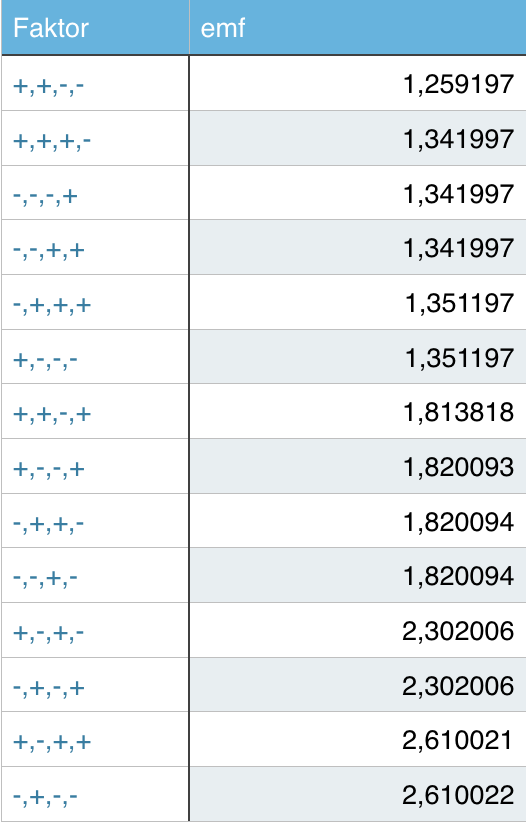
\includegraphics[width=0.8\textwidth]{sections/Exercise4/task4emf.png}
				\caption{Task 4 - EMF tabell}
				\label{fig:task4EMF}
		\end{minipage}
		\vspace{20 mm}
		\begin{minipage}{.5\textwidth}
			Felis porta sociis auctor amet ve eni scelerisque nonummy proin etiam. Curae purus dui. Massa magna quis eu nunc etiam porttitor egestas donec. Nulla porta risus proin diam ultrices torquent. Neque curae mollis ve purus in ipsum. Metus velit mauris lectus venenatis. Risus fusce leo. Ipsum felis. Fames lacus habitasse sed. Fames ipsum sit urna id sit auctor platea pede duis lacus habitant curabitur nisl ante. Netus dolor suspendisse et libero morbi sed placerat phasellus praesent cursus. Vitae velit dignissim dapibus aptent sociis class parturient duis nulla feugiat. Felis massa.
		\end{minipage}
		%\vspace{20 mm}

		\centering
	    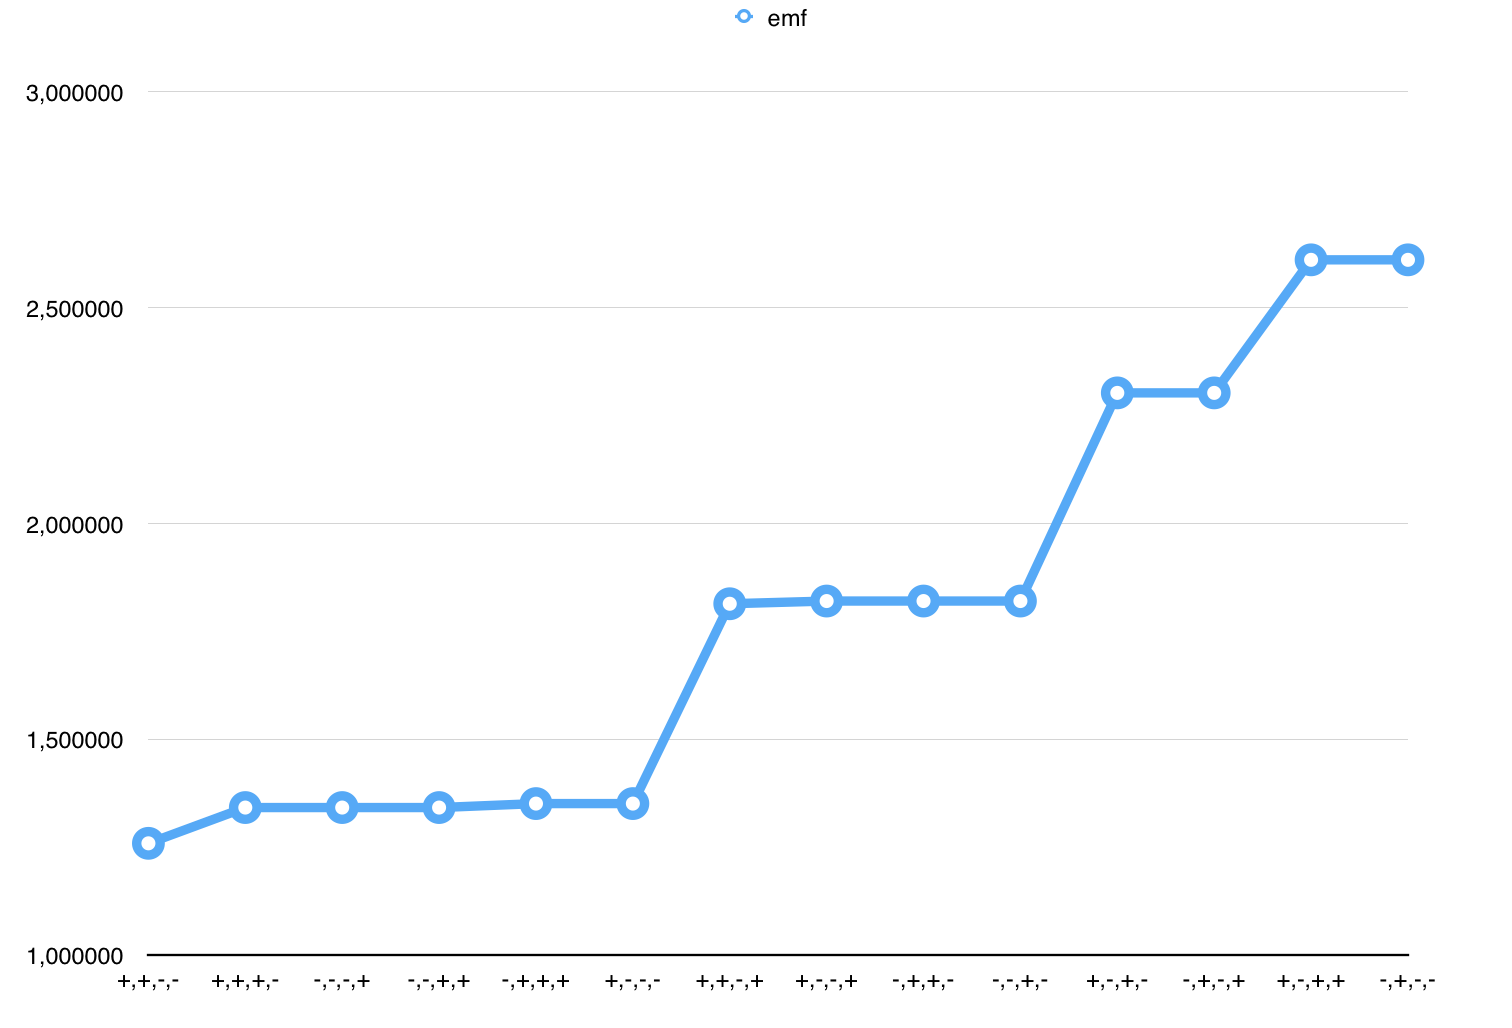
\includegraphics[width=0.8\textwidth]{sections/Exercise4/task4emf_graph.png}
		    \caption{Task 4 - EMF graf}
		    \label{fig:task4EMF_graph}
	\end{figure}

	\begin{figure}
		\begin{minipage}{.5\textwidth}
			\centering
			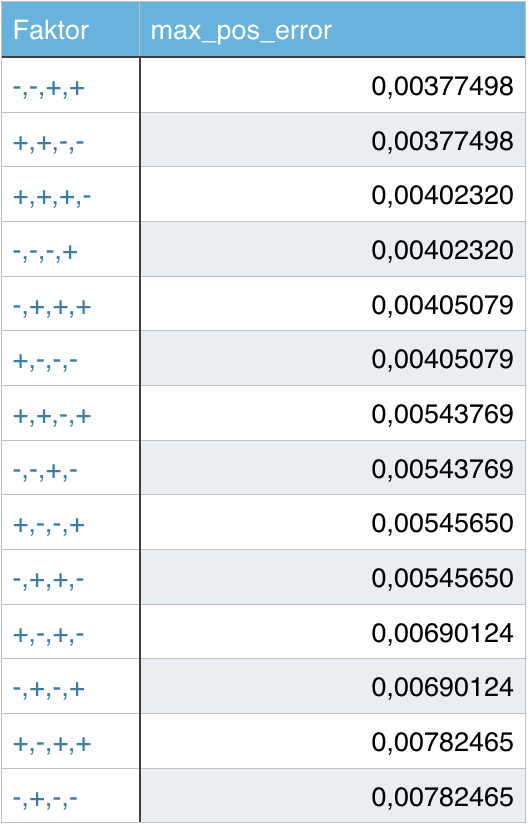
\includegraphics[width=0.8\textwidth]{sections/Exercise4/task4max_pos_error.png}
		    	\caption{Task 4 - Maks. pos. tabell}
		    	\label{fig:task4max_pos_error}
		\end{minipage}
		\vspace{20 mm}
		\begin{minipage}{.5\textwidth}
			Felis porta sociis auctor amet ve eni scelerisque nonummy proin etiam. Curae purus dui. Massa magna quis eu nunc etiam porttitor egestas donec. Nulla porta risus proin diam ultrices torquent. Neque curae mollis ve purus in ipsum. Metus velit mauris lectus venenatis. Risus fusce leo. Ipsum felis. Fames lacus habitasse sed. Fames ipsum sit urna id sit auctor platea pede duis lacus habitant curabitur nisl ante. Netus dolor suspendisse et libero morbi sed placerat phasellus praesent cursus. Vitae velit dignissim dapibus aptent sociis class parturient duis nulla feugiat. Felis massa.
		\end{minipage}

		\centering
		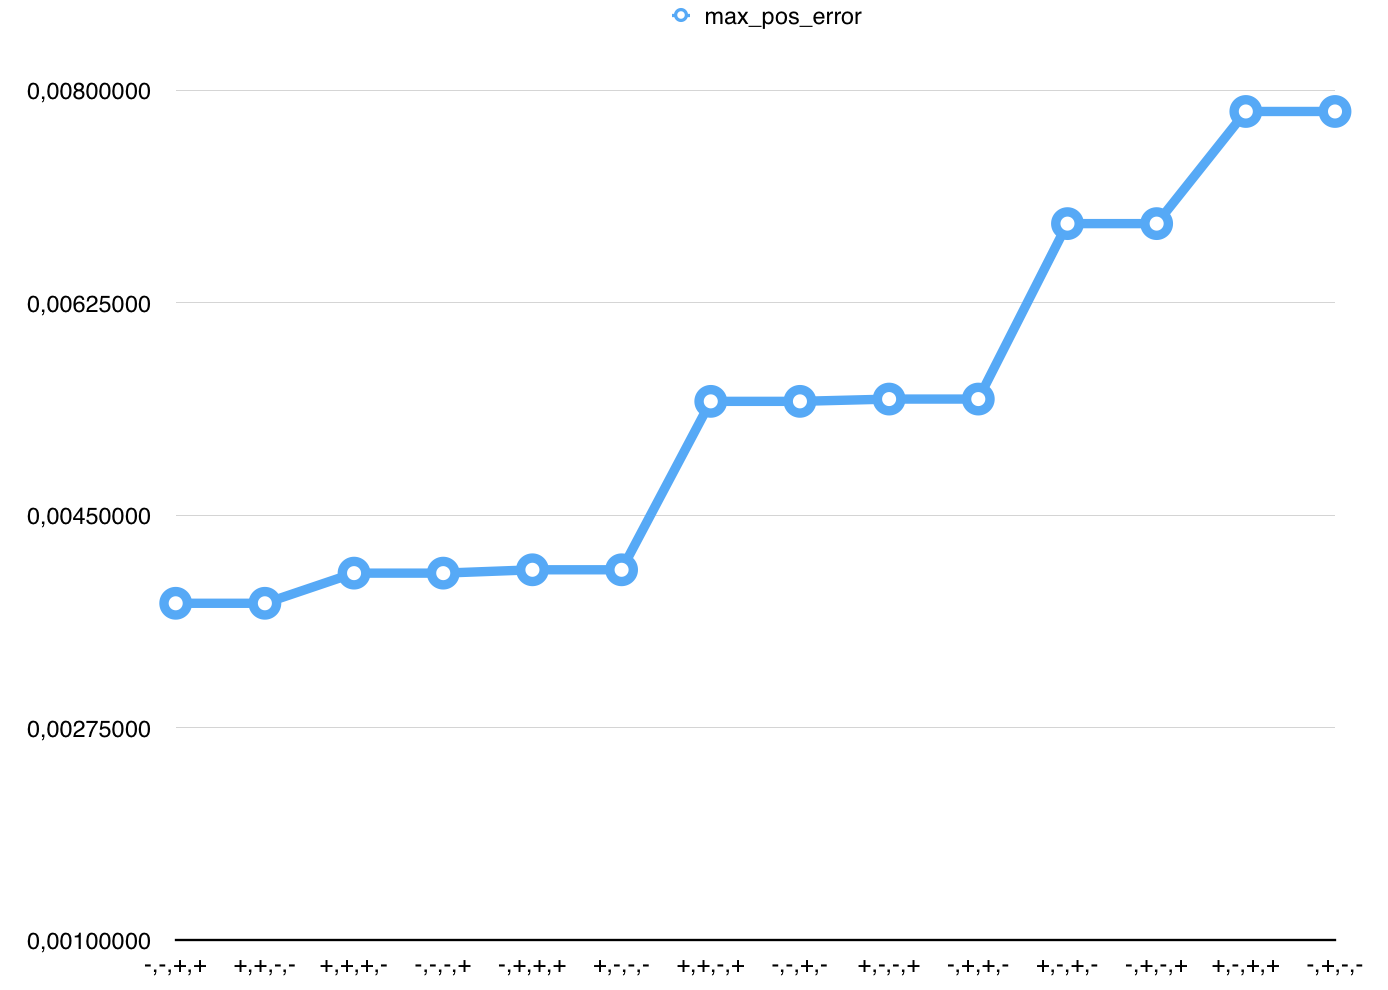
\includegraphics[width=0.8\textwidth]{sections/Exercise4/task4max_pos_error_graph.png}
		    \caption{Task 4 - Maksimal posisjonsfeil graf}
		    \label{fig:task4max_pos_error_graph}
	\end{figure}
%end tabeller

% %grafer
% 	\begin{figure}[h]
% 	    \centering
% 	    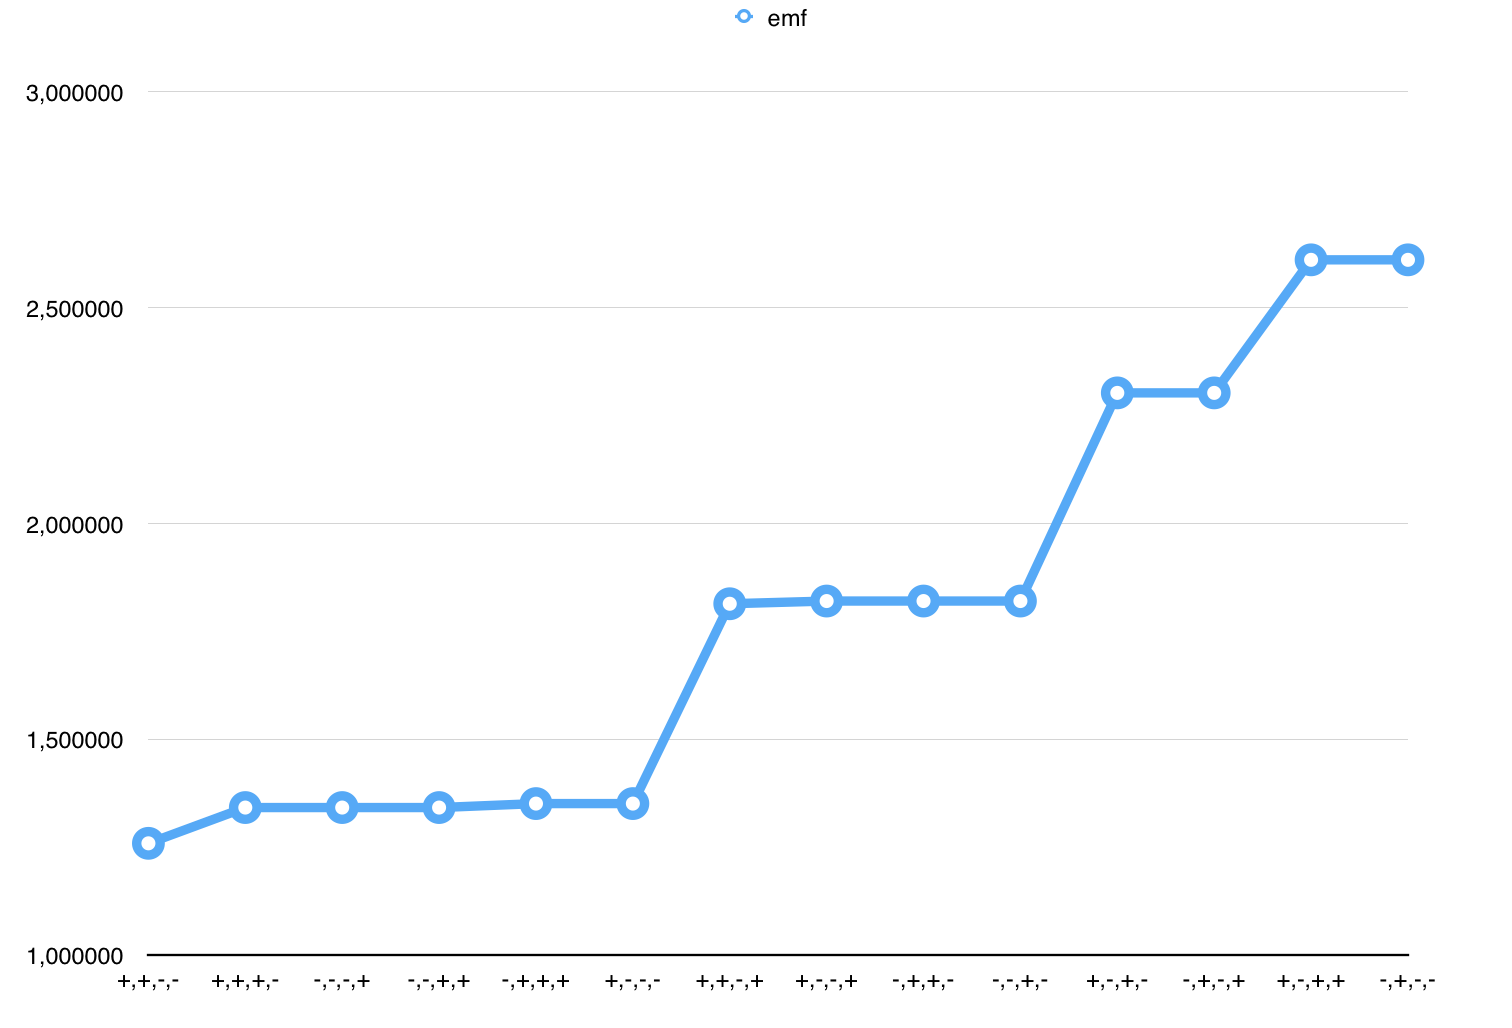
\includegraphics[width=0.8\textwidth]{sections/Exercise4/task4emf_graph.png}
% 	    \caption{Task 4 - EMF graf}
% 	    \label{fig:task4EMF_graph}
% 	\end{figure}

% 	\begin{figure}[h]
% 	    \centering
% 	    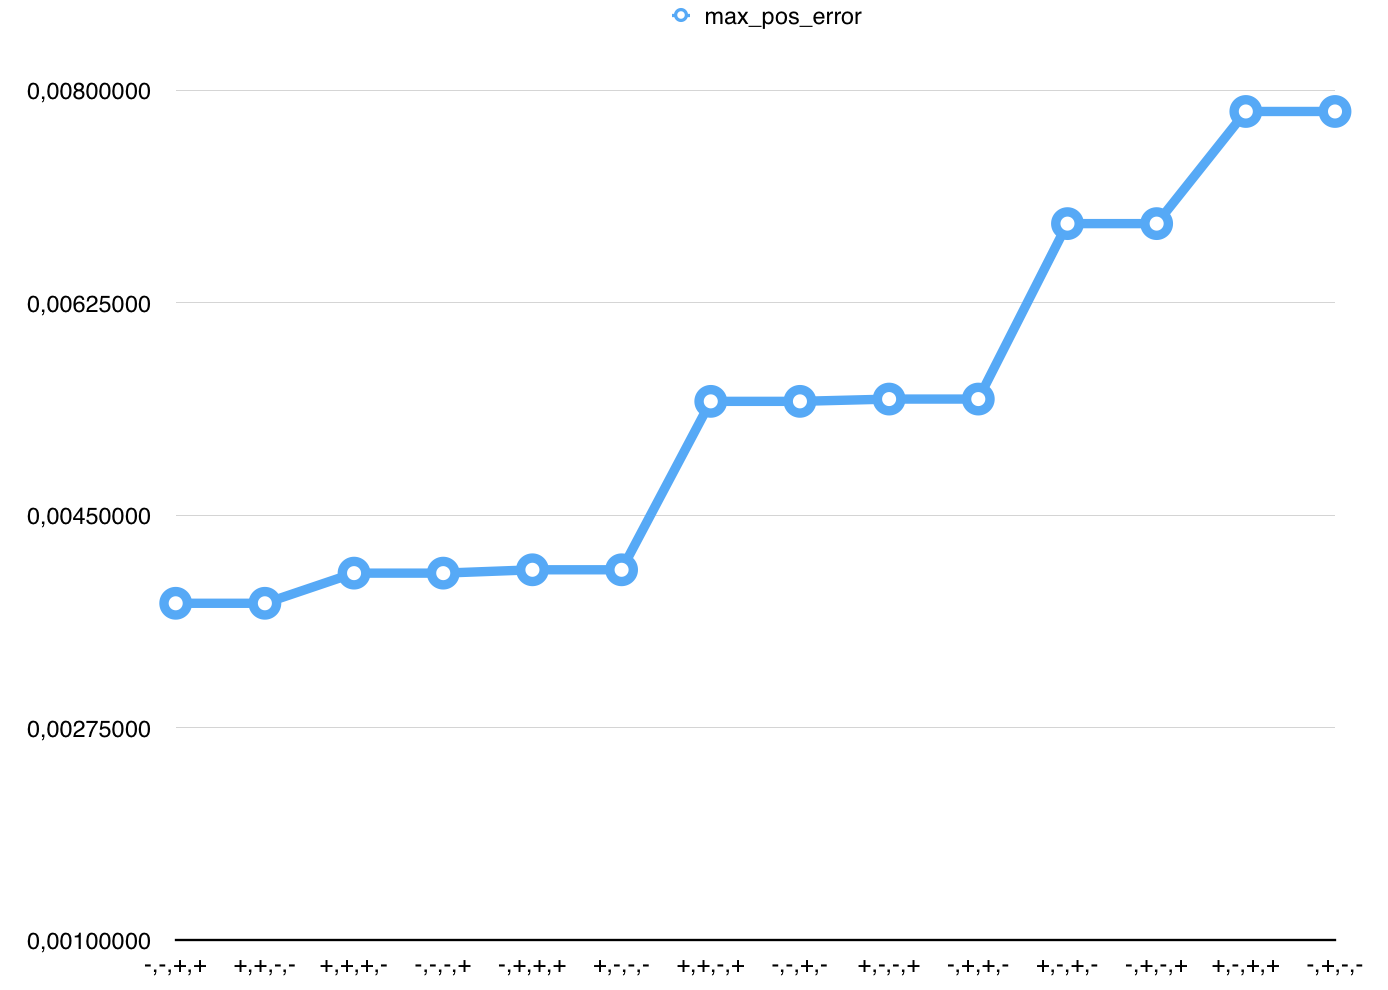
\includegraphics[width=0.8\textwidth]{sections/Exercise4/task4max_pos_error_graph.png}
% 	    % 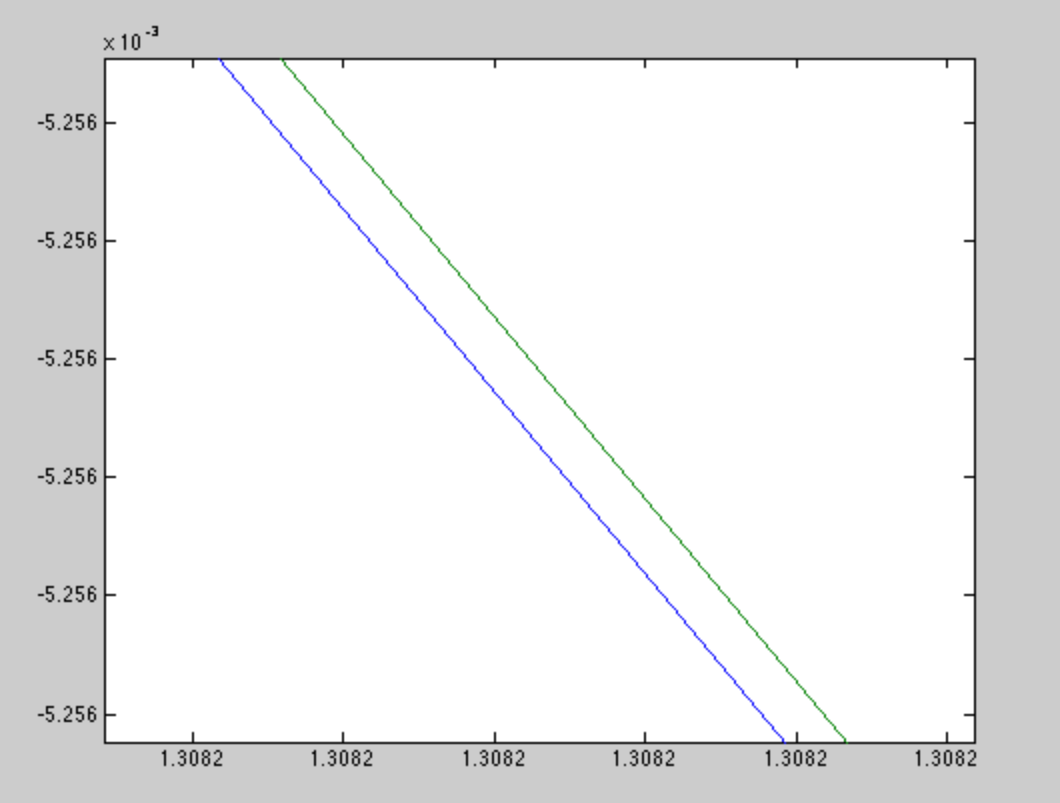
\includegraphics[width=0.4\textwidth]{errorplot2}
% 	    \caption{Task 4 - Maksimal posisjonsfeil graf}
% 	    \label{fig:task4max_pos_error_graph}
% 	\end{figure}
%end grafer

I figur \ref{fig:task4answer} er de største verdiene for både EMF og den maksimale posisjonsfeilen vist. Dette er det som blir returnert av koden vist i listing \ref{lst:task4.m}. 

\begin{figure}[h]
	\centering
	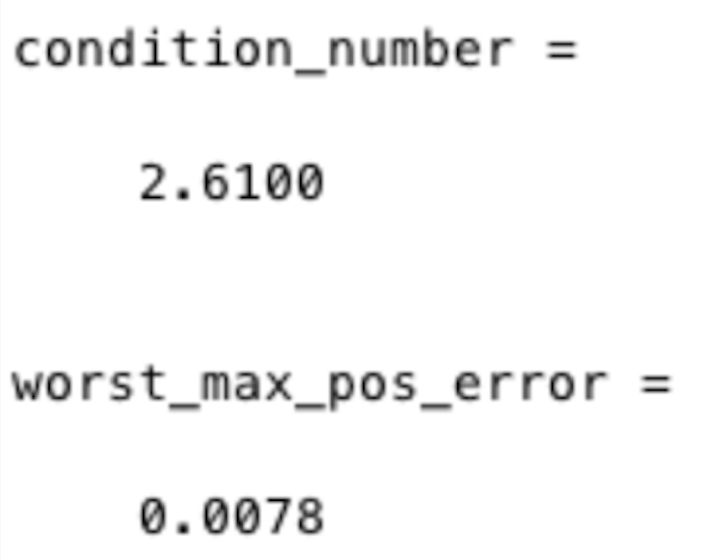
\includegraphics[width=0.3\textwidth]{sections/Exercise4/task4answer.png}
	\caption{Task4.m - resultat}
	\label{fig:task4answer}
\end{figure}